\chapter{Results and Analysis}
\label{chap: results}

In this chapter, we will discuss the performance of a two-emulator setup
built using the default configuration of CL: both the massless- and
massive-neutrino emulators appraised here use the COMET priors
(table~\ref{tab: COMET_priors}), $N_k = 300$, and $N_s = 3000$ for both the
training and testing data sets.

\section{Quantifying the Performance of the Emulator}

To evaluate the performance of the emulator, we use the testing pipeline
explained in section~\ref{sec: test_emu}.
That is, we create an LHS of test cosmologies, which the training stages have
never seen, and compare the output of the emulator object to that of
CAMB. As in neural network contexts, GPR performance is typically evaluated
using test sets (\citealp{Mancini}, \citealp{Arico}, and
\citealp{Eggemeier}).\footnote{However, these test sets are
more commonly referred to as ``validation sets.'' We use the phrase
``test set'' to call to mind the three conventional data sets in a machine
learning setup: training, validation, and testing. This distinction will
prove useful in section~\ref{sec: future_work}.}

We appreciate that appraisal based on test sets
may not provide hard boundaries on the true
range of errors associated with the emulators,
because the continuity of the parameter hypervolume means that an infinite
number of cosmologies could be tested. Therefore, traditional
goodness-of-fit tests such as $\chi^2$ do not apply here.
However, precisely because
power spectra vary smoothly in this space\footnote{Indeed, without this
property, interpolation would be unproductive.}, we expect the error 
curves to vary similarly. So long as the test LHS represents a reasonable
coverage of the parameter space, we expect the errors calculated therefrom to
be similarly representative of emulator performance. On the other
hand, at the edges of the parameter space, where interpolation begins to
break down, the errors will be at their highest, and the following analyses
may not be representative of these edge cases.

For this chapter as well as chapter~\ref{chap: disc_and_conc}, we will focus
on just two error metrics: percent error and squared error. We include percent
error as it is more common in the literature and because it is immediately
interpretable (\citealp{Mancini}, \citealp{Arico}, and
\citealp{Eggemeier}). By contrast, the squared errors are difficult to
understand unless compared across multiple similar cases.
Nevertheless, we argue
that squared errors represent a more useful metric, at least within a single
paper, because they are unbiased with respect to the magnitude of the emulated
quantity. Consider that $P(k)$ is smallest at the largest $k$; if an emulator
mispredicts $P(k)$ with a constant offset, then the percent error curves will
be largest at the smallest $k$. As a further example, consider that the
overall amplitude of $P(k)$ is smaller for smaller $\tilde{\sigma}_{12}$;
if we again imagine a constant offset, $\tilde{\sigma}_{12}$ will appear as a
problematic parameter if we look only at percent error.


\section{Percent and Absolute Errors on Random Cosmologies}

\begin{figure}[ht!]
  \centering
  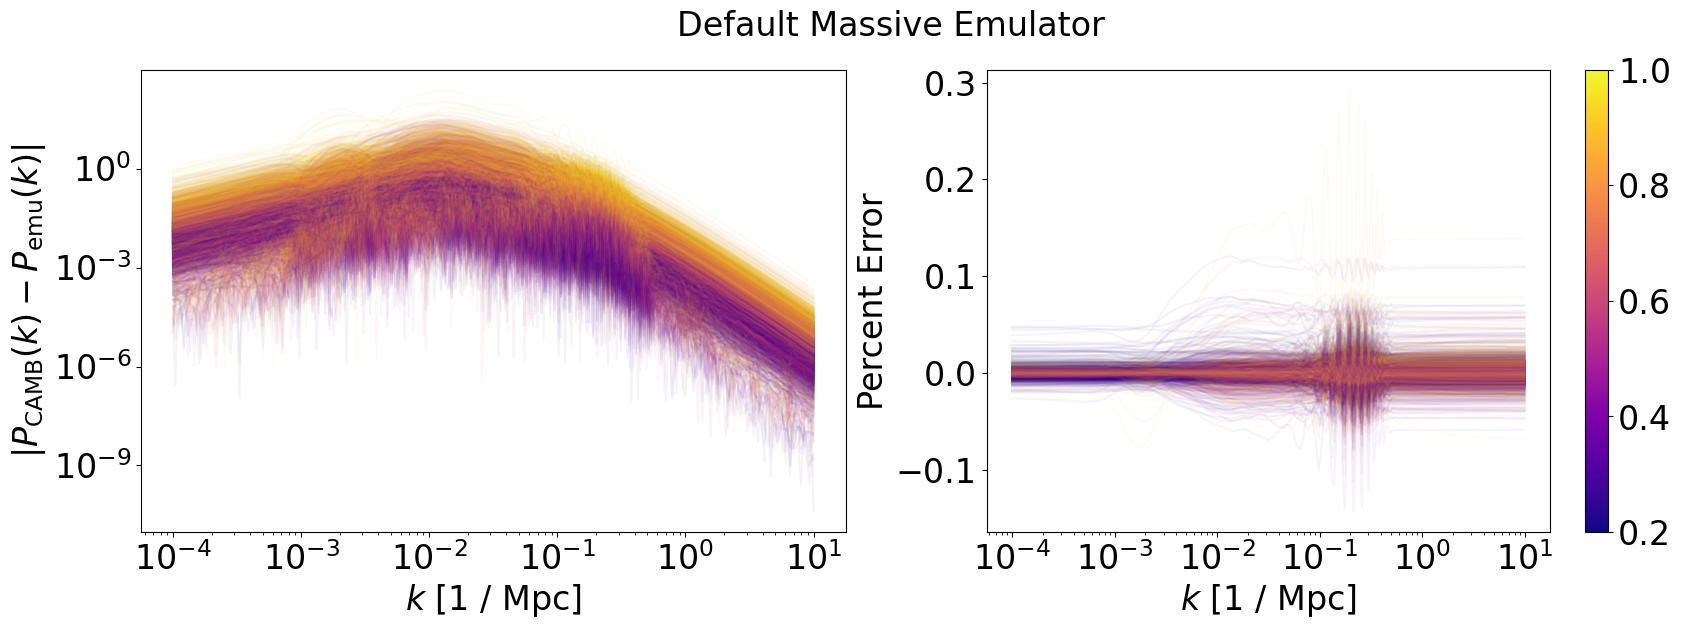
\includegraphics[width=\textwidth]{error_on_emulators/def_massive_curves}
  \caption[Default Massive Emulator Error Curves]{5000 error curves provided 
  by running the test set through the emulator. The curves are colored
  according to their value in $\tilde{\sigma}_{12}$. The opacity of the curves
  allows us to conclude that the dynamic range, at least in the percent
  error case, is dominated by a small number of cosmologies.
  In absolute terms, the emulator
  clearly performs best on the small scales. In relative terms, the
  performance is best on large scales. Regardless of the metric used, the
  error is most extreme on medium scales, and drastic fluctuations can be seen 
  in the percent error plot.}
  \label{fig: def_massive_curves}
\end{figure}

\begin{figure}[ht!]
  \centering
  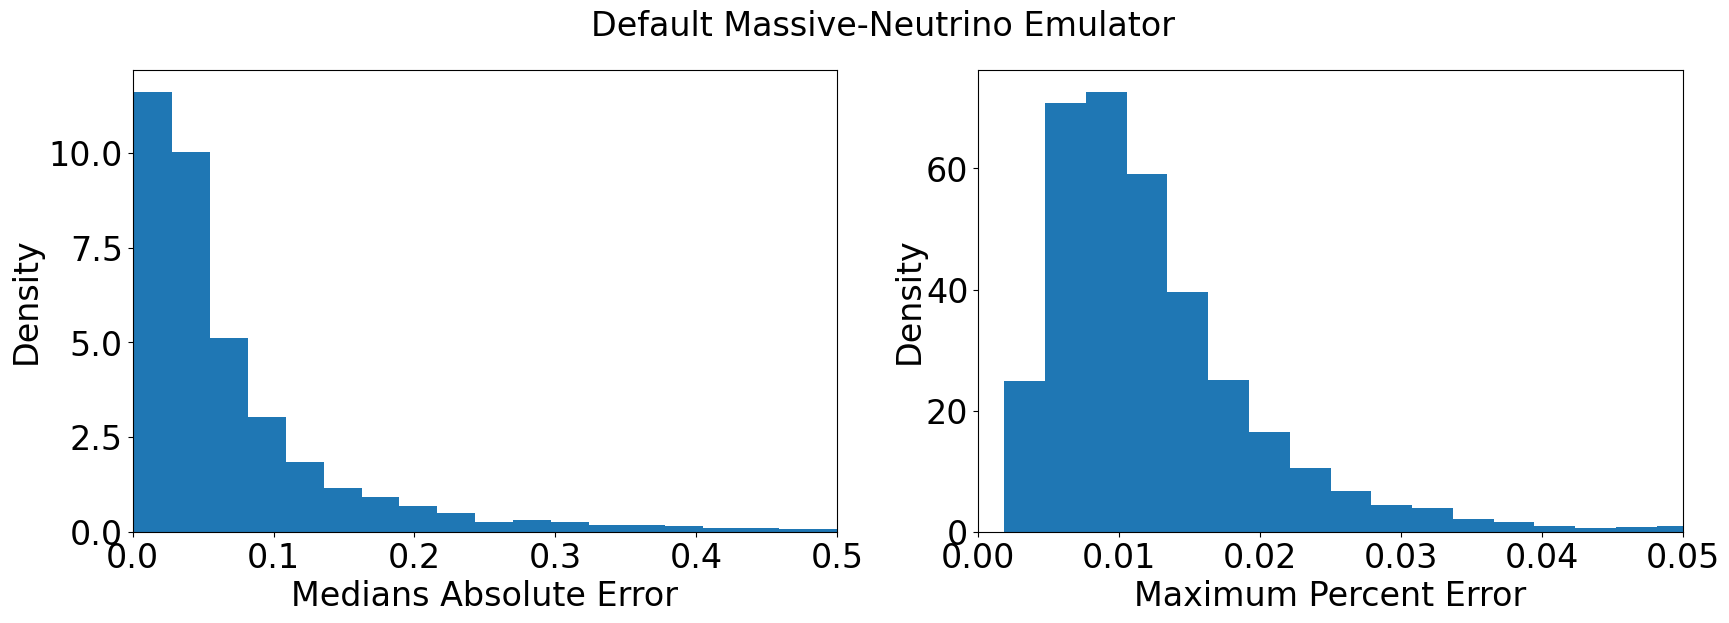
\includegraphics[width=\textwidth]{error_on_emulators/def_massive_hist}
  \caption[Default Massive Emulator Error Histograms]{The left plot is a
  	histogram of the medians of the absolute values of each difference curve.
  	The right plot is a histogram of the maxima of the absolute values of
  	each percent error curve. In both cases, we find the plots to have
  	extremely long tails, so we have truncated these plots at arbitrary
  	right endpoints in order to focus on the central shape.}
  \label{fig: def_massive_hist}
\end{figure}

In figure~\ref{fig: def_massive_curves}, we 
show the performance of the default massive-neutrino emulator. We consider
the overall performance encouraging. Even the worst error curve, which
appears to have been the worst by far, did not exceed a 0.3\% error.
In the follow-up histograms (figure~\ref{fig: def_massive_hist}), we find
that in the vast majority of tested cosmologies, the error does not
exceed 0.04\%.

The curves of figure~\ref{fig: def_massive_curves} were colored according to
their values in $\tilde{\sigma_{12}}$, which we found was the only parameter
associated with a consistent trend. At large scales, lower values of
$\tilde{\sigma}_{12}$ are associated with higher percent errors. However, at
all scales, higher values of $\tilde{\sigma}_{12}$ are strongly tied to
increased absolute error.

The dramatic
oscillations around the BAO region suggest to us that improving the emulator's
handling of the BAO would be the most promising avenue for tightening the
overall distribution of error.

\begin{figure}[ht!]
  \centering
  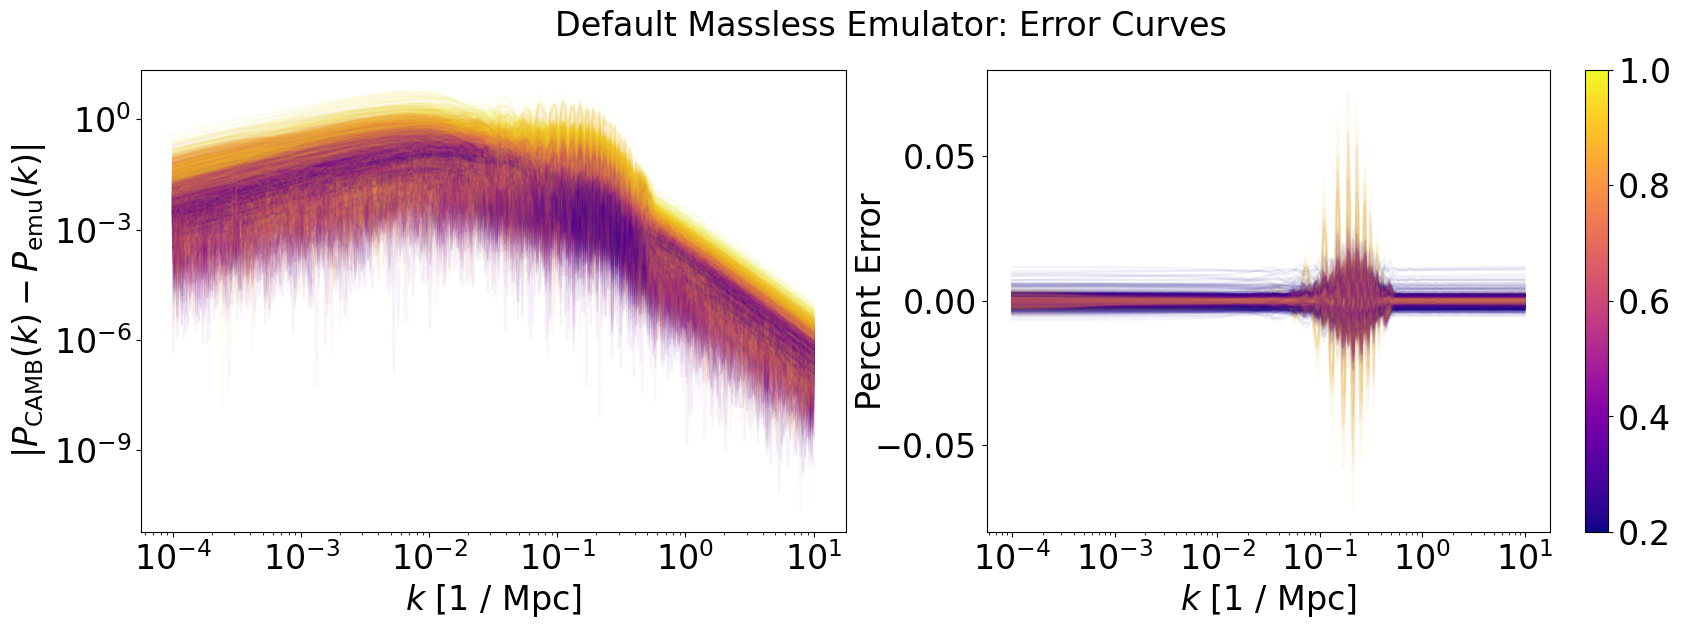
\includegraphics[width=\textwidth]{error_on_emulators/def_massless_curves}
  \caption[Default Massless Emulator Error Curves]{5000 error curves provided 
  by running the test set through the emulator. The curves are colored
  according to their value in $\tilde{\sigma}_{12}$.
  In absolute terms, the emulator
  clearly performs best on the small scales. In relative terms, the
  performance is about the same on large and small scales.
  Regardless of the metric used, the
  error is most extreme on medium scales, and drastic fluctuations can be seen 
  in the percent error plot.}
  \label{fig: def_massless_curves}
\end{figure}

\begin{figure}[ht!]
  \centering
  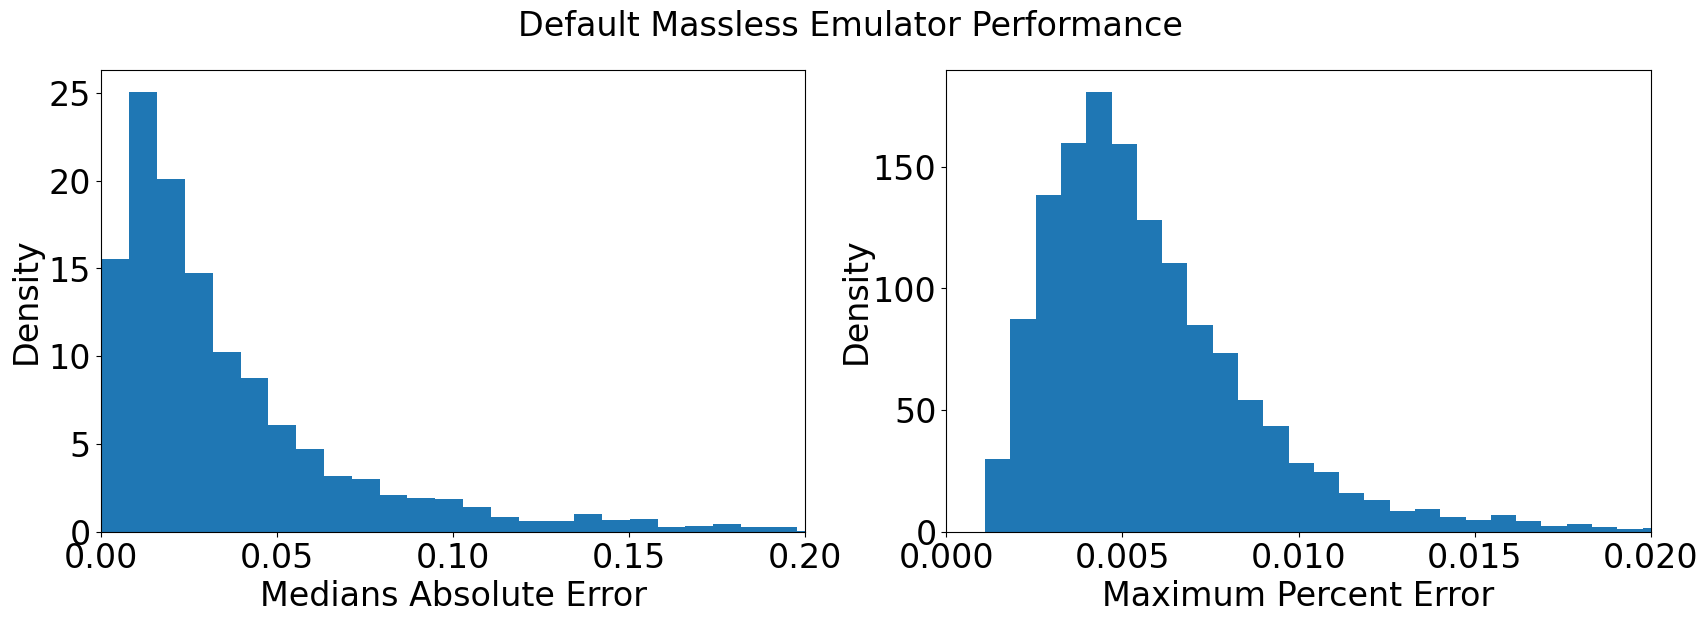
\includegraphics[width=\textwidth]{error_on_emulators/def_massless_hist}
  \caption[Default Massless Emulator Error Histograms]{1000 error curves provided by running the test set through the emulator.}
  \label{fig: def_massless_hist}
\end{figure}

In figures~\ref{fig: def_massless_curves} and~\ref{fig: def_massless_hist},
we have included analogous plots from our massless-neutrino emulator.
The overall shape of the error curves appears similar to the massive
case, although here the absolute errors are small enough that fluctuations
in the BAO region can be clearly seen in both cases. Furthermore, the
percent error curves appear to be tightly concentrated both at small and
large $k$, whereas the spread towards large $k$ increased visibly
in the massive case. From the histograms we can appreciate that the error
distributions are roughly similar but the spread has been tightened in both
histograms by roughly a factor of two. By contrast, the percent error
curves have decreased in dynamic range by a factor of four.

The BAO fluctuations are proportionally much more significant here, suggesting
that the BAO errors are the most significant contributor to percent errors
across all cosmologies. This
further encourages future work to focus on BAO modeling, as both the massive-
and massless-neutrino emulators could benefit significantly.

\textcolor{orange}{Create some plots focusing on the BAO error spikes? i.e.
zoom-in on k-ranges.}

The massive emulator clearly performs worse than its 
massless counterpart. The emulators are difficult to compare because they
were constructed from LHSs of different dimension: four in the massless case,
six in the massive case. Since $N_s = 5000$ is constant, we expect the 
massless LHS to sample the parameter space much more densely than the massive
LHS. In any case, the discrepancy in accuracies will be worsened by the
approximate nature of our fit from section~\ref{sec: proposed_fit}:
the results of section~\ref{sec: fit_testing} indicate
that evolution parameters besides $A_s$ are necessary for complete
characterization of the impact of massive neutrinos. Nevertheless, the
overall percent error of the massive emulator is comparable with that
of CAMB itself, so we consider the massive emulator a confirmation of the
techniques introduced in chapter~\ref{A_s}.

\textcolor{orange}{I plan to spend some time talking 
about \textit{why} parameter x is the current biggest problem for the 
emulator.}

\textcolor{orange}{It would have been nice if you had done like Andrea said,
and produced a plot colored by the ``extremeness'' of the parameters. We
could implement an extremeness index for parameter $x$ simply by taking
subtracting 0.5 and taking the absolute value, assuming that $x$ comes from
the unit LHS. Then, we could take the average over six parameters to get
an extremeness index for the cosmology as a whole. Optionally, for plot
optimization, you could multiply the final value by 2 so that the extremeness
runs from 0 to 1.}


\section{Improvement from Two-emulator Solution}
\label{sec: 2emu_improvement}

\begin{figure}[ht!]
  \centering
  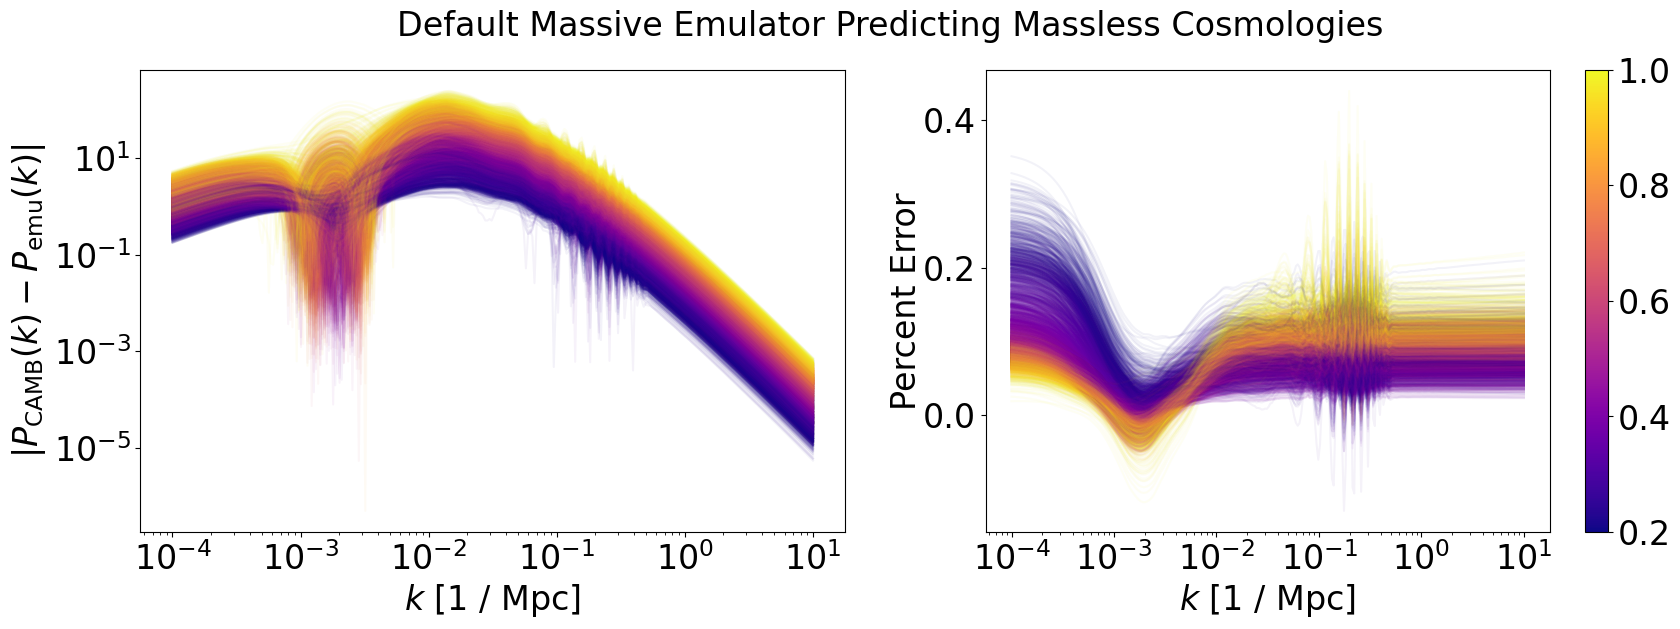
\includegraphics[width=\textwidth]{error_on_emulators/two_emu_curves}
  \caption[Performance of Massive Emulator in Massless Case]{1000 error
  	curves provided
  	by running the massless-neutrino test set through the massive-neutrino 
  	emulator. The shape of both plots is significantly different from the
  	massive-emulator's test cosmologies shown in
  	figure~\ref{fig: def_massive_curves}. We therefore consider our
  	two-emulator solution strongly motivated.}
  \label{fig: two_emu_curves}
\end{figure}

To justify our use of a two-emulator solution to increase
accuracy in the massless-neutrino case, we task the massive-neutrino emulator 
with predictions over the test set of the massless-neutrino emulator.
To adjust the four-dimensional massless-neutrino test LHS to
the six-dimensional massive-neutrino emulator, we filled in
$A_s \approx 2.1272 \cdot 10^{-9}$ and $\omega_\nu = 0$ everywhere.
We consider
this a fair test because we sampled $\omega_\nu$ values for the
massive-neutrino emulator from a uniform distribution [0, 0.01]. Therefore,
in principle, the $\omega_\nu = 0$ case should only be a slight extrapolation.

The overall error of the massive emulator is larger, but this does not
explain all of the results that we see--these error curves also differ
significantly in shape, with increasingly aberrant behavior at large scales.
Also, the BAO feature seems to be slightly complicated by the presence of
massive neutrinos.

Now that we have used the massless-emulator test set to motivate our use of
a two-emulator solution, we move on from the massless emulator.
As evolution-mapping emulation for \textit{massive}-neutrino cosmologies
is the novel feature of this work, we will henceforth concentrate exclusively
on the massive-neutrino emulator.

\section{Minimum Separation of the Training LHC}
\label{sec: error_from_lhc}

% The following plots were generated with emu_experiment_histograms.ipynb
\begin{figure}[ht!]
    \begin{subfigure}{0.35 \textheight}
    \centering
 		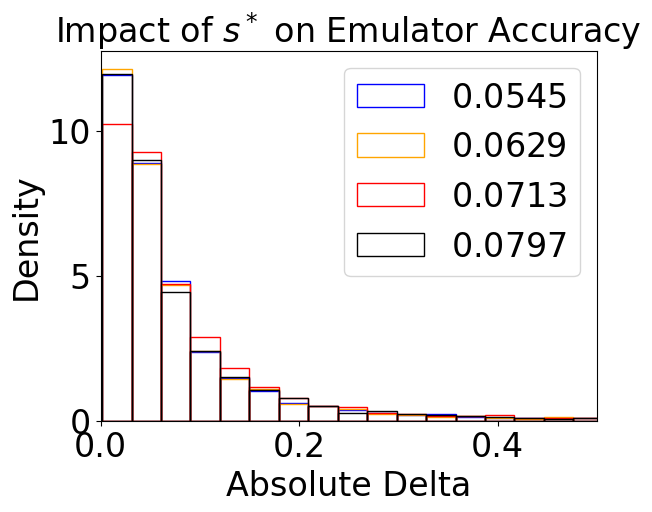
\includegraphics[width=\textwidth]{error_on_emulators/deltas-hist-minsep}
 		\caption{Median absolute errors.}
 		\label{fig: minsep_experiment_deltas}
    \end{subfigure}
    \begin{subfigure}{0.35 \textheight}
    \centering
 		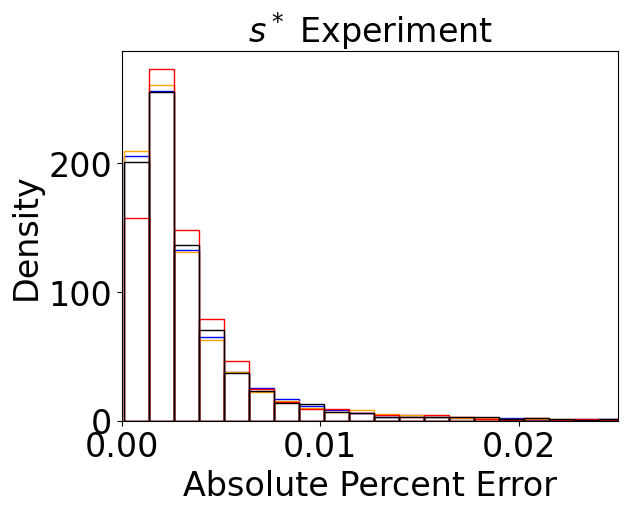
\includegraphics[width=\textwidth]{error_on_emulators/percents-hist-minsep}
 		\caption{Median absolute percent errors.}
 		\label{fig: minsep_experiment_percerr}
    \end{subfigure}
        \centering
    \caption[Impact of $s^*$ on Accuracy]
    		{Histograms of errors associated with emulators trained on LHSs of
    			different $s^*$ values. Despite the theoretical importance of
    			the quantity, its impact on the errors appears extremely limited.}
    \label{fig: minsep_experiment}
\end{figure}

The final training LHS had an $s^*$ of 0.07972 in the massive case and 
0.02274 in the massless case, rounded to four significant figures. In order
to quantitatively explore the impact of the LHS's $s^*$ on the performance
of the emulator, we created three additional emulators of different $s^*$
values and compared their performance using the test set for the default
emulator, which is also the one with the highest $s^*$.

In figure~\ref{fig: minsep_experiment}, we have prepared two histograms to
compare the errors from the four emulators. Surprisingly, $s^*$ does not
appear to affect the error distribution in any distinct way. As a further
step, we include tables~\ref{tab: minsep_experiment_delta_stats}
and~\ref{tab: minsep_experiment_percerr_stats}. None of the columns evolves
in a consistent manner, and so we call the experiment inconclusive.

% The following table was generated with emu_experiment_stats.ipynb
\begin{table}[ht!]
\centering
\begin{tabular}{l|l|l|l|l}
\hline
$s^*$ & Median of Means & Median of Medians & Median of STDs & Maximum PTP \\ \hline
$0.0545$ & 0.167753 & 0.045098 & 0.232575 & 205.656917 \\
$0.0629$ & 0.169627 & 0.044320 & 0.234392 & 174.772714 \\
$0.0713$ & 0.194701 & 0.050606 & 0.275545 & 203.590333 \\
$0.0797$ & 0.173023 & 0.044955 & 0.244320 & 224.434379 \\
\end{tabular}
	\cprotect\caption[$s^*$ Experiment: Percent Error Statistics]{Table of
		absolute error statistics
		when applying the default massless emulator's test
		set to emulators trained on LHSs of different $s^*$ values. In all
		columns, lower values indicate preferred outcomes. ``STD:'' standard
		deviation. ``PTP:'' peak-to-peak, or the difference in the maximum
		and minimum values. None of the columns shows a consistent trend.
		Only in the case of the median of medians is the last-row value
		lower than that of the first row.}
 \label{tab: minsep_experiment_delta_stats}
\end{table}

% The following table was generated with emu_experiment_stats.ipynb
\begin{table}[ht!]
\centering
\begin{tabular}{l|l|l|l|l}
\hline
$s^*$ & Median of Means & Median of Medians & Median of STDs & Maximum PTP \\ \hline
$0.0545$ & 0.002835 & 0.002240 & 0.002025 & 0.192945 \\
$0.0629$ & 0.002850 & 0.002179 & 0.002079 & 0.196711 \\
$0.0713$ & 0.003052 & 0.002409 & 0.002059 & 0.266151 \\
$0.0797$ & 0.002883 & 0.002255 & 0.002058 & 0.291348 \\
\end{tabular}
	\cprotect\caption[$s^*$ Experiment: Percent Error Statistics]{Table of
		absolute percent error statistics
		when applying the default massless emulator's test
		set to emulators trained on LHSs of different $s^*$ values. In all
		columns, lower values indicate preferred outcomes. ``STD:'' standard
		deviation. ``PTP:'' peak-to-peak, or the difference in the maximum
		and minimum values. None of the columns shows an expected trend.
		We consider it a coincidence that the maximum PTP in percent error
		\textit{increases} consistently with increasing $s^*$, especially
		since the corresponding column in the absolute errors
		(see table~\ref{tab: minsep_experiment_delta_stats}) lacks this
		trend.}
 \label{tab: minsep_experiment_percerr_stats}
\end{table}

As mentioned in section~\ref{sec: lhc}, we expected the errors to consistently
decrease with increasing $s^*$, as this quantity communicates the evenness of 
the coverage of the space of cosmologies.

The tested range in $s^*$ may have been too small for us to appreciate a
consistent impact. The scope of this experiment was limited by our approach
to generating LHCs, as the smallest and largest $s^*$ values tested came at
the cost of several days of computation time. Alternatively, we may have been
able to detect a consistent difference in the emulators by expanding the
testing set with many more cosmologies. For example, if we test over
30000 cosmologies (instead of the 5000 used here), we may find that noise in
our random selection of cosmologies obscures the effect of $s^*$.

Despite these two suggestions, we nevertheless conclude that the impact of
$s^*$ may be extremely weak, even if a higher $s^*$ value is theoretically
preferred. This suggests that our brute-force solution of randomly generating
LHSs is appropriate for our purposes.


\section{Resolution of the k Axis}

\begin{figure}[ht!]
  \centering
  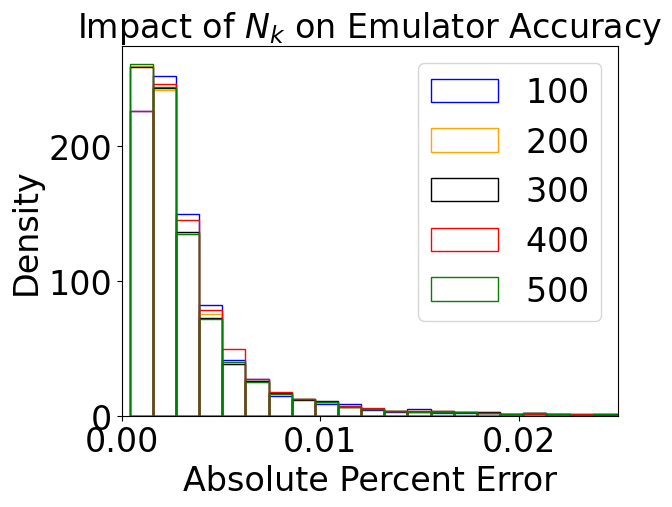
\includegraphics[scale=0.5]{error_on_emulators/percents-hist-N_k}
  \caption[Impact of $N_k$ on Accuracy]{The test is too fair!}
  \label{fig: Nk_experiment}
\end{figure}

To understand the impact of our choice of $N_k = 300$ for the emulator, we
also constructed and tested emulators for $N_k = 100$, 200, 400, and 500.
To control for interpolation error, each emulator has its own test set where
the test spectra have the same $N_k$. The
difference in test sets contributes random error that obscures the comparison.
We are interested in whether our GPR infrastructure is less efficient at
learning lower- than higher-resolution spectra.

The absolute errors cannot be directly compared across different emulators.
This is because the $N_k = 500$ emulator is tested at five times as many
points as the $N_k = 100$ emulator. Consequently, for this section, we focus
exclusively on percent errors.

In figure~\ref{fig: Nk_experiment}, we show a histogram of the median absolute
percent errors. The histograms are difficult to distinguish and do not admit
of an immediate preference for any $N_k$ value. Again, we produce a summary
of relevant statistics in table~\ref{tab: Nk_experiment_percerr_stats}. As
with our study of the impact of $s^*$, the values within each column do not
vary widely from each other, and do not confrom to any consistent trend.

% The following table was generated with emu_experiment_stats.ipynb
\begin{table}[ht!]
\centering
\begin{tabular}{l|l|l|l|l}
\hline
$N_k$ & Median of Means & Median of Medians & Median of STDs & Maximum PTP \\ \hline
$100$ & 0.003082 & 0.002427 & 0.002174 & 0.272042 \\
$200$ & 0.002878 & 0.002243 & 0.002054 & 0.297159 \\
$300$ & 0.002883 & 0.002255 & 0.002058 & 0.291348 \\
$400$ & 0.003034 & 0.002461 & 0.002042 & 0.277015 \\
$500$ & 0.002881 & 0.002221 & 0.002088 & 0.296367 \\
\end{tabular}
	\cprotect\caption[$N_k$ Experiment: Percent Error Statistics]{Median of
		absolute percent errors.}
 \label{tab: Nk_experiment_percerr_stats}
\end{table}

Unlike with $s^*$, we lack a theoretical basis for believing $N_k$ to be a
quantity important to the performance of the emulator. Instead, the value of
$N_k$ should be modified by the user according to the use case. However, we
caution that our results here cannot be interpreted as conclusive evidence
against $N_k$'s relevance. Our inconclusive results from the $s^*$ experiment
suggest that our tests are not sufficiently thorough to establish a
hyperparameter's relevance, because in that case we have a strong theoretical
basis for the parameter's importance.

\section{Number of Training Samples}
\label{sec: num_samples}

\textcolor{blue}{Justify choice of 5000 samples for each: maybe we can make a
trend plot showing diminishing returns in test error?}

% The following plots were generated with emu_experiment_histograms.ipynb
\begin{figure}[ht!]
    \begin{subfigure}{0.35 \textheight}
    \centering
 		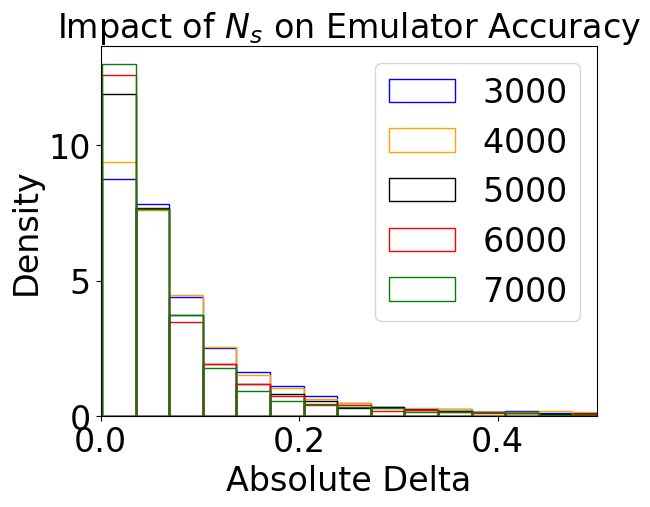
\includegraphics[width=\textwidth]{error_on_emulators/deltas-hist-N_s}
 		\caption{Median absolute errors.}
 		\label{fig: Ns_experiment_deltas}
    \end{subfigure}
    \begin{subfigure}{0.35 \textheight}
    \centering
 		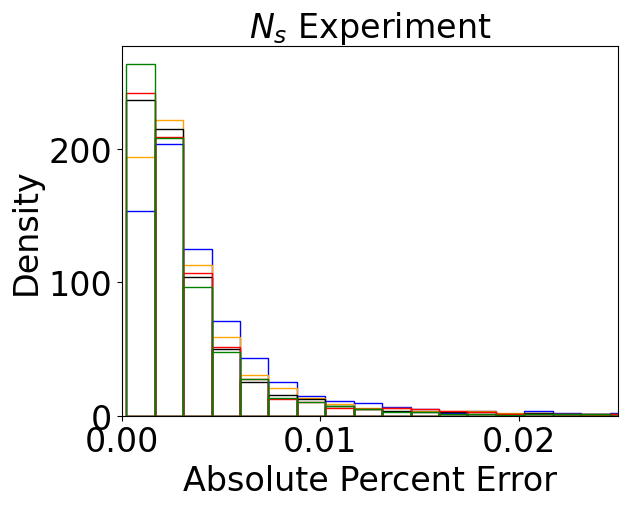
\includegraphics[width=\textwidth]{error_on_emulators/percents-hist-N_s}
 		\caption{Median absolute percent errors.}
 		\label{fig: Ns_experiment_percerr}
    \end{subfigure}
        \centering
    \caption[Impact of $s^*$ on Accuracy]
    		{Histograms of errors associated with emulators trained on LHSs of
    			different $N_s$ values. Doesn't seem to make much difference,
    			but unlike the other cases, we can definitely say here that it
    			makes a difference.}
    \label{fig: Ns_experiment}
\end{figure}

% The following table was generated with emu_experiment_stats.ipynb
\begin{table}[ht!]
\centering
\begin{tabular}{l|l|l|l|l}
\hline
$N_s$ & Median of Means & Median of Medians & Median of STDs & Maximum PTP \\ \hline
$3000$ & 0.2382 & 0.0588 & 0.3388 & 175.5588 \\
$4000$ & 0.2010 & 0.0567 & 0.2741 & 185.5470 \\
$5000$ & 0.1730 & 0.0450 & 0.2443 & 224.4344 \\
$6000$ & 0.1712 & 0.0425 & 0.2415 & 146.6090 \\
$7000$ & 0.1633 & 0.0410 & 0.2305 & 118.7862 \\
\end{tabular}
	\cprotect\caption[$N_s$ Experiment: Deltas Statistics]{This table shows
		the volatility of the last column, as the median colmuns agree on the
		trend.}
 \label{tab: Ns_experiment_deltas_stats}
\end{table}

% The following table was generated with emu_experiment_stats.ipynb
\begin{table}[ht!]
\centering
\begin{tabular}{l|l|l|l|l}
\hline
$N_s$ & Median of Means & Median of Medians & Median of STDs & Maximum PTP \\ \hline
$3000$ & 0.0037 & 0.0030 & 0.0027 & 0.2794 \\
$4000$ & 0.0032 & 0.0026 & 0.0022 & 0.2305 \\
$5000$ & 0.0029 & 0.0023 & 0.0021 & 0.2913 \\
$6000$ & 0.0028 & 0.0022 & 0.0020 & 0.1893 \\
$7000$ & 0.0027 & 0.0021 & 0.0019 & 0.1189 \\
\end{tabular}
	\cprotect\caption[$N_s$ Experiment: Percent Error Statistics]{YES!
		We caution that the last column can be a misleading statistic
		(especially because the deltas table does not show the same trend), but
		it is still a helpful value to quote...}
 \label{tab: Ns_experiment_percerr_stats}
\end{table}


% This might go better in the CassL section, but I think I ought to motivate 
% the decision to use 5000 training arrays.

\textcolor{orange}{I'll have to concede that the results of this section are 
not entirely comprehensive; we didn't train any emulators over the 
uncertainties of analogous validation hypercubes. All comparisons here use the
simpler pipeline of just two data sets, training and testing.}
